\section{\gls{DPR} for Internal Fault Mitigation}\label{InternalFaults}
\begin{figure}
    \resizebox{\columnwidth}{!}{\tikzset{every picture/.style={line width=0.25pt}} %set default line width to 0.75pt        

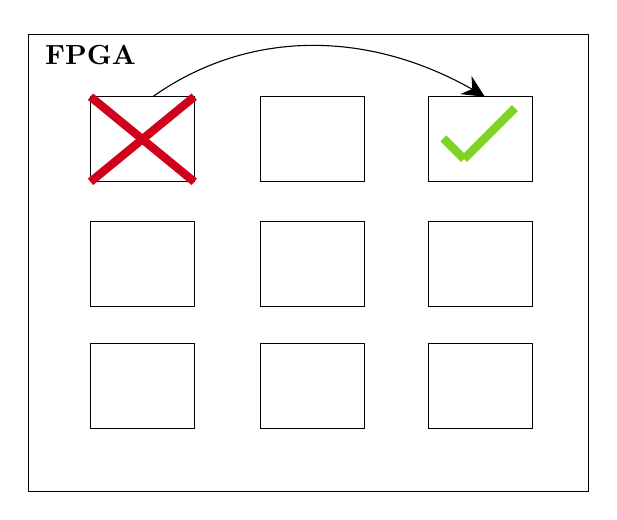
\begin{tikzpicture}[x=0.75pt,y=0.75pt,yscale=-1,xscale=1]
%uncomment if require: \path (0,279); %set diagram left start at 0, and has height of 279

%Shape: Rectangle [id:dp5787797491333819] 
\draw   (6,20) -- (276,20) -- (276,240) -- (6,240) -- cycle ;
%Shape: Rectangle [id:dp17505095690594463] 
\draw   (36,50) -- (86,50) -- (86,91) -- (36,91) -- cycle ;
%Shape: Rectangle [id:dp3058047377979807] 
\draw   (36,110) -- (86,110) -- (86,151) -- (36,151) -- cycle ;
%Shape: Rectangle [id:dp004684645465554249] 
\draw   (36,169) -- (86,169) -- (86,210) -- (36,210) -- cycle ;
%Shape: Rectangle [id:dp3077757040785931] 
\draw   (118,50) -- (168,50) -- (168,91) -- (118,91) -- cycle ;
%Shape: Rectangle [id:dp7450799349257811] 
\draw   (118,110) -- (168,110) -- (168,151) -- (118,151) -- cycle ;
%Shape: Rectangle [id:dp2725857150503048] 
\draw   (118,169) -- (168,169) -- (168,210) -- (118,210) -- cycle ;
%Shape: Rectangle [id:dp3816815123242099] 
\draw   (199,50) -- (249,50) -- (249,91) -- (199,91) -- cycle ;
%Shape: Rectangle [id:dp2885393682660524] 
\draw   (199,110) -- (249,110) -- (249,151) -- (199,151) -- cycle ;
%Shape: Rectangle [id:dp4969175268738504] 
\draw   (199,169) -- (249,169) -- (249,210) -- (199,210) -- cycle ;
%Straight Lines [id:da8580754234796655] 
\draw [color={rgb, 255:red, 208; green, 2; blue, 27 }  ,draw opacity=1 ][line width=3]    (36,50) -- (86,91) ;


%Straight Lines [id:da5772916268060835] 
\draw [color={rgb, 255:red, 208; green, 2; blue, 27 }  ,draw opacity=1 ][line width=3]    (86,50) -- (36,91) ;


%Curve Lines [id:da5702734861080319] 
\draw    (66,50) .. controls (112.04,17.33) and (171.3,17) .. (224.39,49.02) ;
\draw [shift={(226,50)}, rotate = 211.67000000000002] [fill={rgb, 255:red, 0; green, 0; blue, 0 }  ][line width=0.75]  [draw opacity=0] (10.72,-5.15) -- (0,0) -- (10.72,5.15) -- (7.12,0) -- cycle    ;

%Straight Lines [id:da7282259837027933] 
\draw [color={rgb, 255:red, 126; green, 211; blue, 33 }  ,draw opacity=1 ][line width=3]    (240.5,55.5) -- (216,80) ;


%Straight Lines [id:da7142424530641487] 
\draw [color={rgb, 255:red, 126; green, 211; blue, 33 }  ,draw opacity=1 ][line width=3]    (216,80) -- (206,70) ;



% Text Node
\draw (36,30) node  [align=left] {\textbf{FPGA}};


\end{tikzpicture}
}
    \caption{Internal Fault Mitigation - functionality from a faulty tile is moved to a healthy area with \gls{DPR}}\label{fig:internalFaultMitigation}
\end{figure}
%\tikzset{every picture/.style={line width=0.25pt}} %set default line width to 0.75pt        

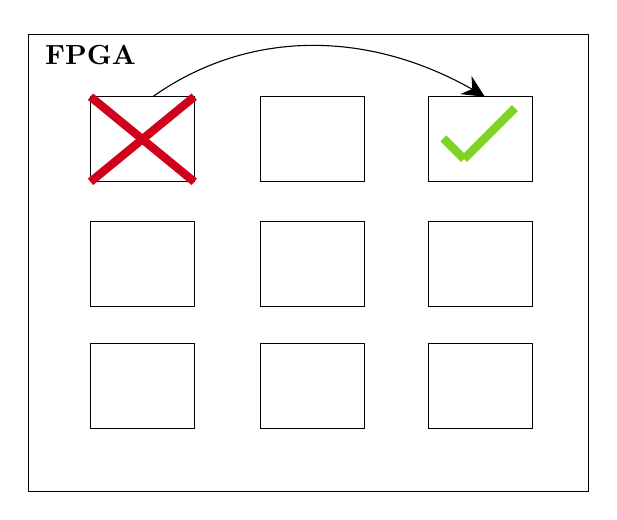
\begin{tikzpicture}[x=0.75pt,y=0.75pt,yscale=-1,xscale=1]
%uncomment if require: \path (0,279); %set diagram left start at 0, and has height of 279

%Shape: Rectangle [id:dp5787797491333819] 
\draw   (6,20) -- (276,20) -- (276,240) -- (6,240) -- cycle ;
%Shape: Rectangle [id:dp17505095690594463] 
\draw   (36,50) -- (86,50) -- (86,91) -- (36,91) -- cycle ;
%Shape: Rectangle [id:dp3058047377979807] 
\draw   (36,110) -- (86,110) -- (86,151) -- (36,151) -- cycle ;
%Shape: Rectangle [id:dp004684645465554249] 
\draw   (36,169) -- (86,169) -- (86,210) -- (36,210) -- cycle ;
%Shape: Rectangle [id:dp3077757040785931] 
\draw   (118,50) -- (168,50) -- (168,91) -- (118,91) -- cycle ;
%Shape: Rectangle [id:dp7450799349257811] 
\draw   (118,110) -- (168,110) -- (168,151) -- (118,151) -- cycle ;
%Shape: Rectangle [id:dp2725857150503048] 
\draw   (118,169) -- (168,169) -- (168,210) -- (118,210) -- cycle ;
%Shape: Rectangle [id:dp3816815123242099] 
\draw   (199,50) -- (249,50) -- (249,91) -- (199,91) -- cycle ;
%Shape: Rectangle [id:dp2885393682660524] 
\draw   (199,110) -- (249,110) -- (249,151) -- (199,151) -- cycle ;
%Shape: Rectangle [id:dp4969175268738504] 
\draw   (199,169) -- (249,169) -- (249,210) -- (199,210) -- cycle ;
%Straight Lines [id:da8580754234796655] 
\draw [color={rgb, 255:red, 208; green, 2; blue, 27 }  ,draw opacity=1 ][line width=3]    (36,50) -- (86,91) ;


%Straight Lines [id:da5772916268060835] 
\draw [color={rgb, 255:red, 208; green, 2; blue, 27 }  ,draw opacity=1 ][line width=3]    (86,50) -- (36,91) ;


%Curve Lines [id:da5702734861080319] 
\draw    (66,50) .. controls (112.04,17.33) and (171.3,17) .. (224.39,49.02) ;
\draw [shift={(226,50)}, rotate = 211.67000000000002] [fill={rgb, 255:red, 0; green, 0; blue, 0 }  ][line width=0.75]  [draw opacity=0] (10.72,-5.15) -- (0,0) -- (10.72,5.15) -- (7.12,0) -- cycle    ;

%Straight Lines [id:da7282259837027933] 
\draw [color={rgb, 255:red, 126; green, 211; blue, 33 }  ,draw opacity=1 ][line width=3]    (240.5,55.5) -- (216,80) ;


%Straight Lines [id:da7142424530641487] 
\draw [color={rgb, 255:red, 126; green, 211; blue, 33 }  ,draw opacity=1 ][line width=3]    (216,80) -- (206,70) ;



% Text Node
\draw (36,30) node  [align=left] {\textbf{FPGA}};


\end{tikzpicture}

\glspl{FPGA} provide high flexibility and good performance in many areas that require a high amount of concurrent computing and therefore benefit from a dedicated hardware implementation.
These properties prove useful for applications in the domain of aerospace and help to reduce the cost for satellites and spacecraft while providing high flexibility throughout the development process. 

But \glspl{FPGA} are especially vulnerable to cosmic radiation which can create a multitude of internal errors in the \gls{FPGA} and thereby breaking its intended functionality \cite{ito_total_2015}.
While there are radiation hardened \glspl{FPGA} available on the market, the mass of a space embedded system is still composed of 80\% radiation shielding \cite{ito_total_2015}.
Yet, this shielding is still not able to provide sufficient protection from radiation induced errors, especially on long term missions. 
Therefore, solutions for fault mitigation in aerospace \glspl{FPGA} need to be developed on the architectural level instead of the physical level. 
This may also provide the advantage of lower requirements for radiation shielding and therefore a reduced cost for payload on rocket launches.

The next section reviews the different types of faults and categorizes them. 

\subsection{Types of Internal Faults}
There are different types of faults that may occur in the lifetime of an \gls{FPGA}, a short overview over the most relevant ones is given in the following.
\par
\textbf{Transient Faults}
\begin{itemize}
    \item \glspl{SEU}, e.g. radiation induced \cite{alkady_fault-tolerant_2014}, \cite{lee_fault-tolerant_2017}
    \begin{itemize}
    \item Change of logic state in memory cell
    \item Commonly tackled by redundancy
    \item Built-in fault detection unit possible
    \end{itemize}
    \item Single Bit Errors (SBEs)
    \item Single Event Transients (SETs)
    \item Address Decoding Faults
\end{itemize}

Faults occur either in the interconnect of the \gls{FPGA} (which uses up to 80\% of the available silicon) or in its actual logic blocks \cite{alkady_fault-tolerant_2014}, \cite{jing_huang_routability_2004}.
\par
\textbf{Permanent Faults}
\begin{itemize}
    \item Time Dependant Dielectric Breakdowns (TDDBs)
    \item Electro Migration
    \item Hot Carrier Effect
\end{itemize}

Based on this review, two main categories of errors emerge.
Firstly, \textit{permanent faults} (also known as \textit{hard errors}), which include all faults that render the affected area completely unusable. 
Secondly, \textit{transient faults} (also known as \textit{soft errors}), which encompasses faults where a reclamation of the erroneous area may still be possible after the initial mitigation process.

\gls{DPR} allows for recovery from both categories. Different recovery strategies are introduced in the next section. 

\subsection{Mitigation Strategies for Internal Faults}\label{MitigationOfInternalFaults}
To mitigate the aforementioned internal faults in an \gls{FPGA}, different strategies can be employed.
All of them feature \gls{DPR} as a means to move functional blocks from a faulty silicon area to a healthy one.
What sets them apart is the way of fault detection and the specifically employed \gls{DPR} strategy.

This section is going to introduce the most common concepts and how they are applied. 

The work in \cite{sharma_run-time_2018} proposes not only ways for fault recovery, but also ways of maintaining as much functionality as possible under varying power constraints. 
\gls{DPR} is utilized to achieve \gls{RT-SA}, i.e. a system that can dynamically alter its architecture to mitigate the effect of changed circumstances.
